\documentclass{beamer}

\usetheme[sectionpage=simple, subsectionpage=simple,
numbering=fraction, progressbar=none]
{metropolis}

\usepackage[utf8]{inputenc}
\usepackage{graphicx}
\graphicspath{{./img/}}
\usepackage{tikz}

\title{Testing Hypothesis}
\date{\today}
\author{Gonzalo G. Peraza Mues}
% \institute{Universidad Politécnica de Yucatán}

\titlegraphic{
\includegraphics[height=1.5cm]{logo-upy}}

\newcommand{\E}[1]{\operatorname{E}\left[#1\right]}
\newcommand{\Var}[1]{\operatorname{Var}\left(#1\right)}
\newcommand{\abs}[1]{\left|#1\right|}
\renewcommand{\P}[1]{P\left(#1\right)}


\begin{document}
\maketitle
\begin{frame}{Non numerical inference. Choosing between two hypothesis}
  Useful when we need to choose between two conflicting theories.

  Examples:
  \begin{itemize}
  \item assess whether the lifetime of a certain type of ball bearing deviates
    or does not deviate from the lifetime guaranteed by the manufacturer
  \item an engineer wants to know whether dry drilling is faster or the same as
    wet drilling
  \item a gynecologist wants to find out whether smoking affects or does not
    affect the probability of getting pregnant
  \item the Allied Forces want to know whether the German war production is
    equal to or smaller than what Allied intelligence agencies reported
  \end{itemize}
\end{frame}

\begin{frame}{A war example: Allied intelligence reports on German war production.}

  Problem: Reported production was a lot higher than was observed by serial
  numbers:
  \begin{itemize}
  \item   Observed serial numbers: 61 19 56 24 16.
  \item   Reported production: 350 tanks.
  \end{itemize}


  We want to choose between two propositions:
  \begin{itemize}
  \item \alert{Null Hypothesis $H_0$}: $N=350$.
  \item \alert{Alternative Hypothesis $H_1$}: $N<350$.
  \end{itemize}
  If we reject $H_0$, we accept $H_1$. $H_1$ must be chosen carefully. Options:
  $N \neq 350$, $N > 350$.
\end{frame}

\begin{frame}[t]{Quick exercises}
  In the drilling example, suppose the data on drill times for dry drilling are
  modeled as a realization of a random sample from a distribution with
  expectation $\mu_1$, and similarly the data for wet drilling correspond to a
  distribution with expectation $\mu_2$. We want to know whether dry drilling is
  faster than wet drilling. To this end we test the null hypothesis
  $H_0 : \mu_1 = \mu_2$ (the drill time is the same for both methods). What
  would you choose for $H_1$?
\end{frame}

\begin{frame}{To decide whether $H_0$ is false we use a statistical model.}
  \alert{Test Statistic}: Suppose the dataset is modeled as the realization of
  random variables $X_1.X_2,\ldots, X_n$. A test statistic is any sample
  statistic $T = h(X_1,X_2,\ldots,X_n)$, whose numerical value is used to
  decide whether we reject $H_0$.
\end{frame}

\begin{frame}{Statistical model}
  Serial numbers are modeled as a realization of random variables
  $X_1,X_2,\ldots, X_5$ representing five draws without replacement from the
  numbers $1,2,\ldots,N$.
  \begin{align*}
    \text{\alert{Test statistic:}}T = \text{max}\{X_1,X_2,\ldots,X_5\}.\\
    \E{T} = n\frac{N+1}{n+1} = \frac{5}{6}(N+1)
  \end{align*}
  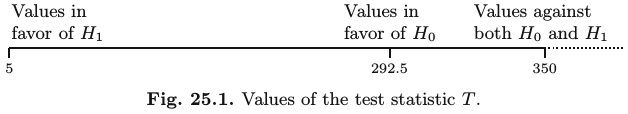
\includegraphics[width=\linewidth]{test-statistic}

  From the data: $t=\text{max}\{61, 19, 56, 24, 16\} = 61$
\end{frame}

\begin{frame}[t]{Quick exercise}
  Another possible test statistic would be $\bar{X}_5$. If we use its values as
  a credibility scale for $H_0$, then what are the possible values of
  $\bar{X}_5$, which values of $\bar{X}_5$ are in favor of $H_1$: $N<350$, and
  which values are in favor of $H_0$: $N=350$?
\end{frame}

\begin{frame}{Tail probabilities}
  Can we reach the conclusion that $H_0$ is false beyond reasonable doubt?

  Values of T that provide stronger evidence against H0 than 61 are to the left
  of 61.

  \begin{align*}
    \P{T\leq 61} = \P{\text{max}\{ X_1,X_2,\ldots,X_5 \}}\\
    = \frac{61}{350}\frac{60}{349}\frac{59}{348}\frac{58}{347}\frac{57}{346}
    = 0.0014
  \end{align*}
  This probability is so small that we view the value 61 as strong evidence
  against the null hypothesis.

  \alert{The tail probability expresses how likely it is to obtain a value of
    the test statistic T at least as extreme as the value t observed for the
    data. Such a probability is called a p-value. }
\end{frame}

\begin{frame}[t]{Quick exercise}
  Suppose that the Allied intelligence agencies had reported a production of 80
  tanks, so that we would test $H_0:N=80$ against $H_1:N<80$. Compute the
  p-value corresponding to 61. Would you conclude $H_0$ is false beyond
  reasonable doubt?
\end{frame}
  
\begin{frame}{Type I and Type II Errors}
  \begin{center}
    \begin{tabular}{l|cc}
      &$H_0$ is true&$H_1$ is true\\\hline
      Reject $H_0$&Type I error&Correct decision \\
      Not reject $H_0$&Correct decision&Type II error
    \end{tabular}
  \end{center}
  
  What amount of risk one is willing to take to falsely reject $H_0$?

  As a rule of thumb \alert{0.05} is used as the level where reasonable doubt
  begins.

  \begin{center}
    \textbf{\alert{Always report the p-value.}}
  \end{center}
\end{frame}

\begin{frame}[t]{Quick exercise}
  Suppose we adopt the following decision rule about the null hypothesis:
  ``reject $H_0:N=350$ whenever $T\leq 250$.'' Using this decision rule, what is
  the probability of committing a type I error?
\end{frame}

\end{document}


%%% Local Variables:
%%% mode: latex
%%% TeX-master: t
%%% End:
